% SPDX-FileCopyrightText: 2023 Iegor Riepin, Tom Brown
%
% SPDX-License-Identifier: CC-BY-4.0

\lipsum[1]


\subsection{Signal 1: quality of local renewable resources}

\begin{figure*}
    \centering
    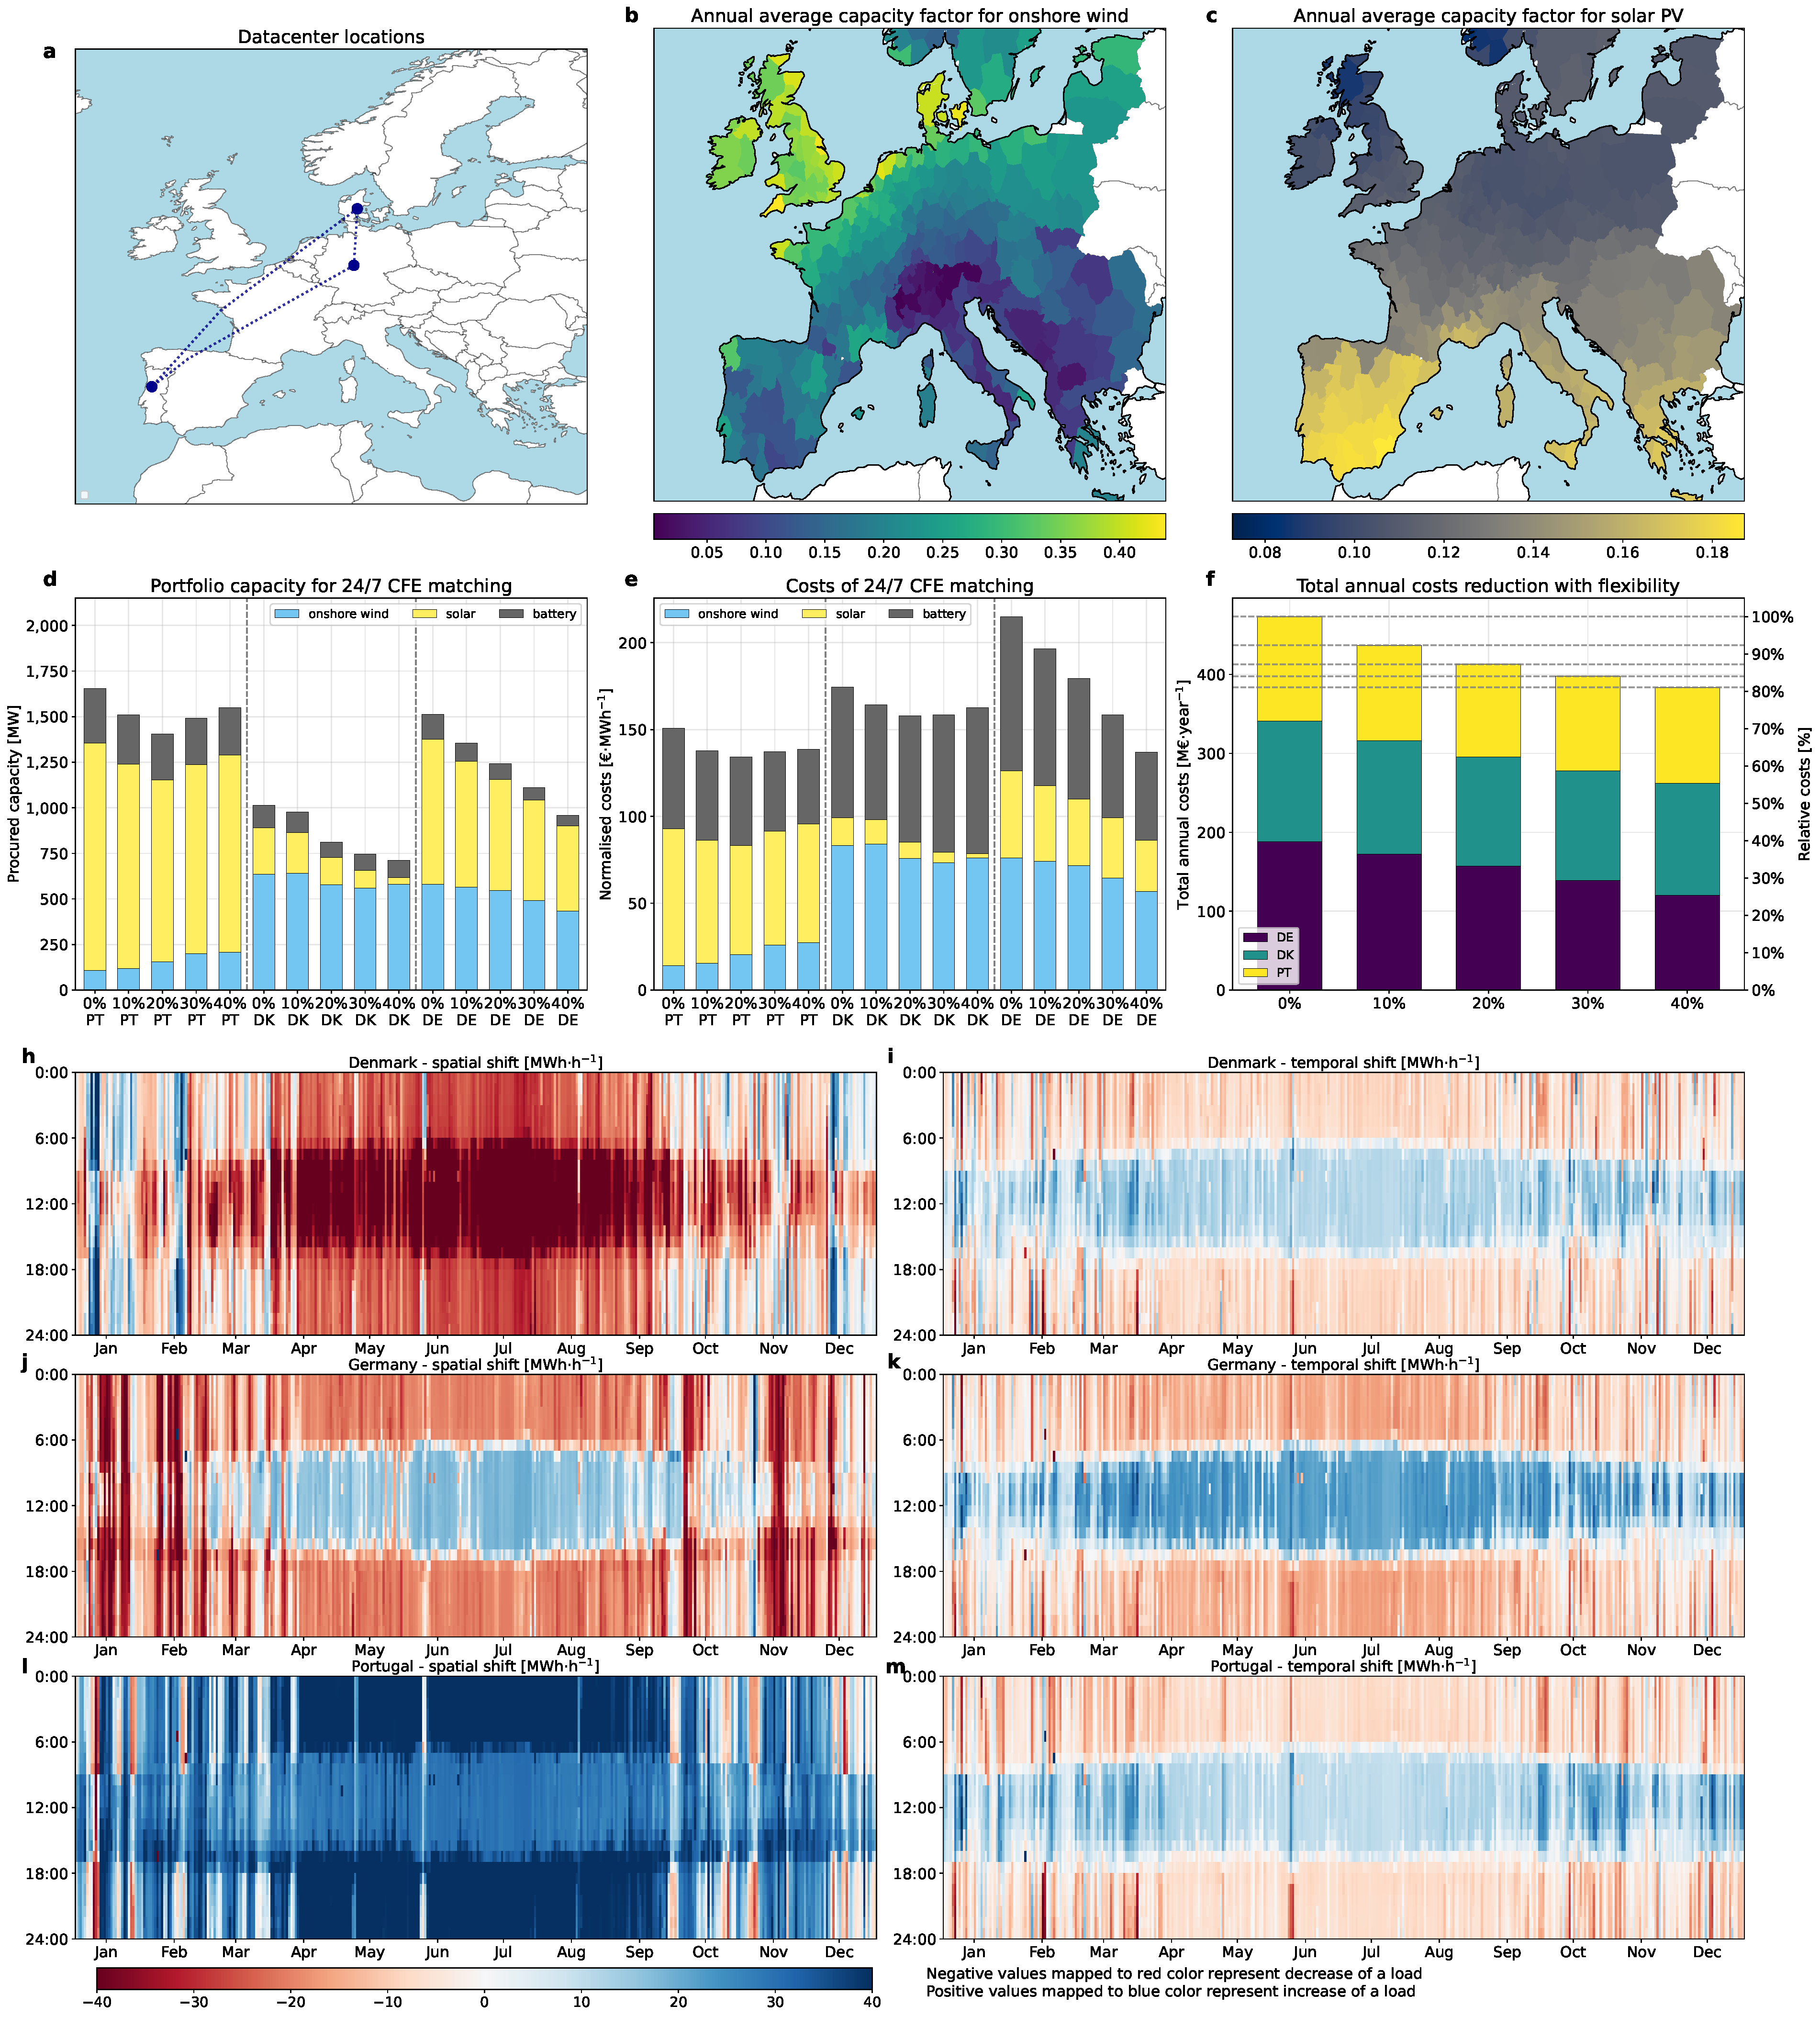
\includegraphics[width=\textwidth]{img/dashboard.pdf}
    \caption{Illustration of the signal 1: quality of local renewable resources.
        \textbf{a:} Assumed datacenter locations: Denmark, Germany, Portugal.
        \textbf{b,c:} Annual average capacity factor of onshore wind and solar photovoltaic. Data is simulated using the ERA5 reanalysis dataset for weather year 2013 and aggregated to 256 regions in Europe.
        \textbf{d:} Cost-optimal portfolio of renewable resources and battery storage sufficient for 24/7 matching. Steps on x-axis represent increasing share of flexible load.
        \textbf{e:} Cost breakdown of 24/7 matching strategy.
        \textbf{f:} Total annual costs of 24/7 matching strategy as a function load flexibility. Relative axis is normalized to the costs of inflexible load.
        \textbf{h,j,l:} Hourly spatial load shifts for the three datacenter locations. Color mapping represents the quantity of load \enquote{received} from other locations or \enquote{sent} away.
        \textbf{i,k,m:} Hourly temporal load shifts for the three datacenter locations. Color mapping represents the quantity of load shifted to a given hour from other times, or shifted from a given hour to another time.}
    \label{fig: dashboard1}
\end{figure*}


\subsection{Signal 2: low correlation of wind power generation over long distances}

\begin{figure*}
    \centering
    \includegraphics[width=\textwidth]{img/dashboard_2.png}
    \caption{Illustration of the signal 2: low correlation of wind power generation over long distances.
    \textbf{a:} Assumed datacenter locations: pairwise connections across regions with similar quality of renewable resources. Here: Ireland with Northern Ireland, or England, or the Netherlands, or Denmark (-west zone).
    \textbf{b,c:} Peason correlation of hourly capacity factor for onshore wind generation, if Denmark (-west zone, panel b) or selected region of Ireland (panel c) are taken as basis. As a result of different weather conditions, wind feed-in has a noticeable correlation falloff over distances of 300-400 km. Data is simulated using the ERA5 reanalysis dataset for weather year 2013 and aggregated to 256 regions in Europe.
    \textbf{d} Hourly spatial load shifts for the selected scenario and datacenter; here datacenter is located Denmark (and another one is located Ireland). Color mapping represents the quantity of load \enquote{received} from other locations or \enquote{sent} away.
    \textbf{e} Cost savings of 24/7 matching with increasing distance between datacenters. Costs are normalized to the cost level of inflexible load.}
    \label{fig:dashboard2}
\end{figure*}


\subsection{Signal 3: time lag in solar radiation peaks due to Earth's rotation}

\begin{figure*}
    \centering
    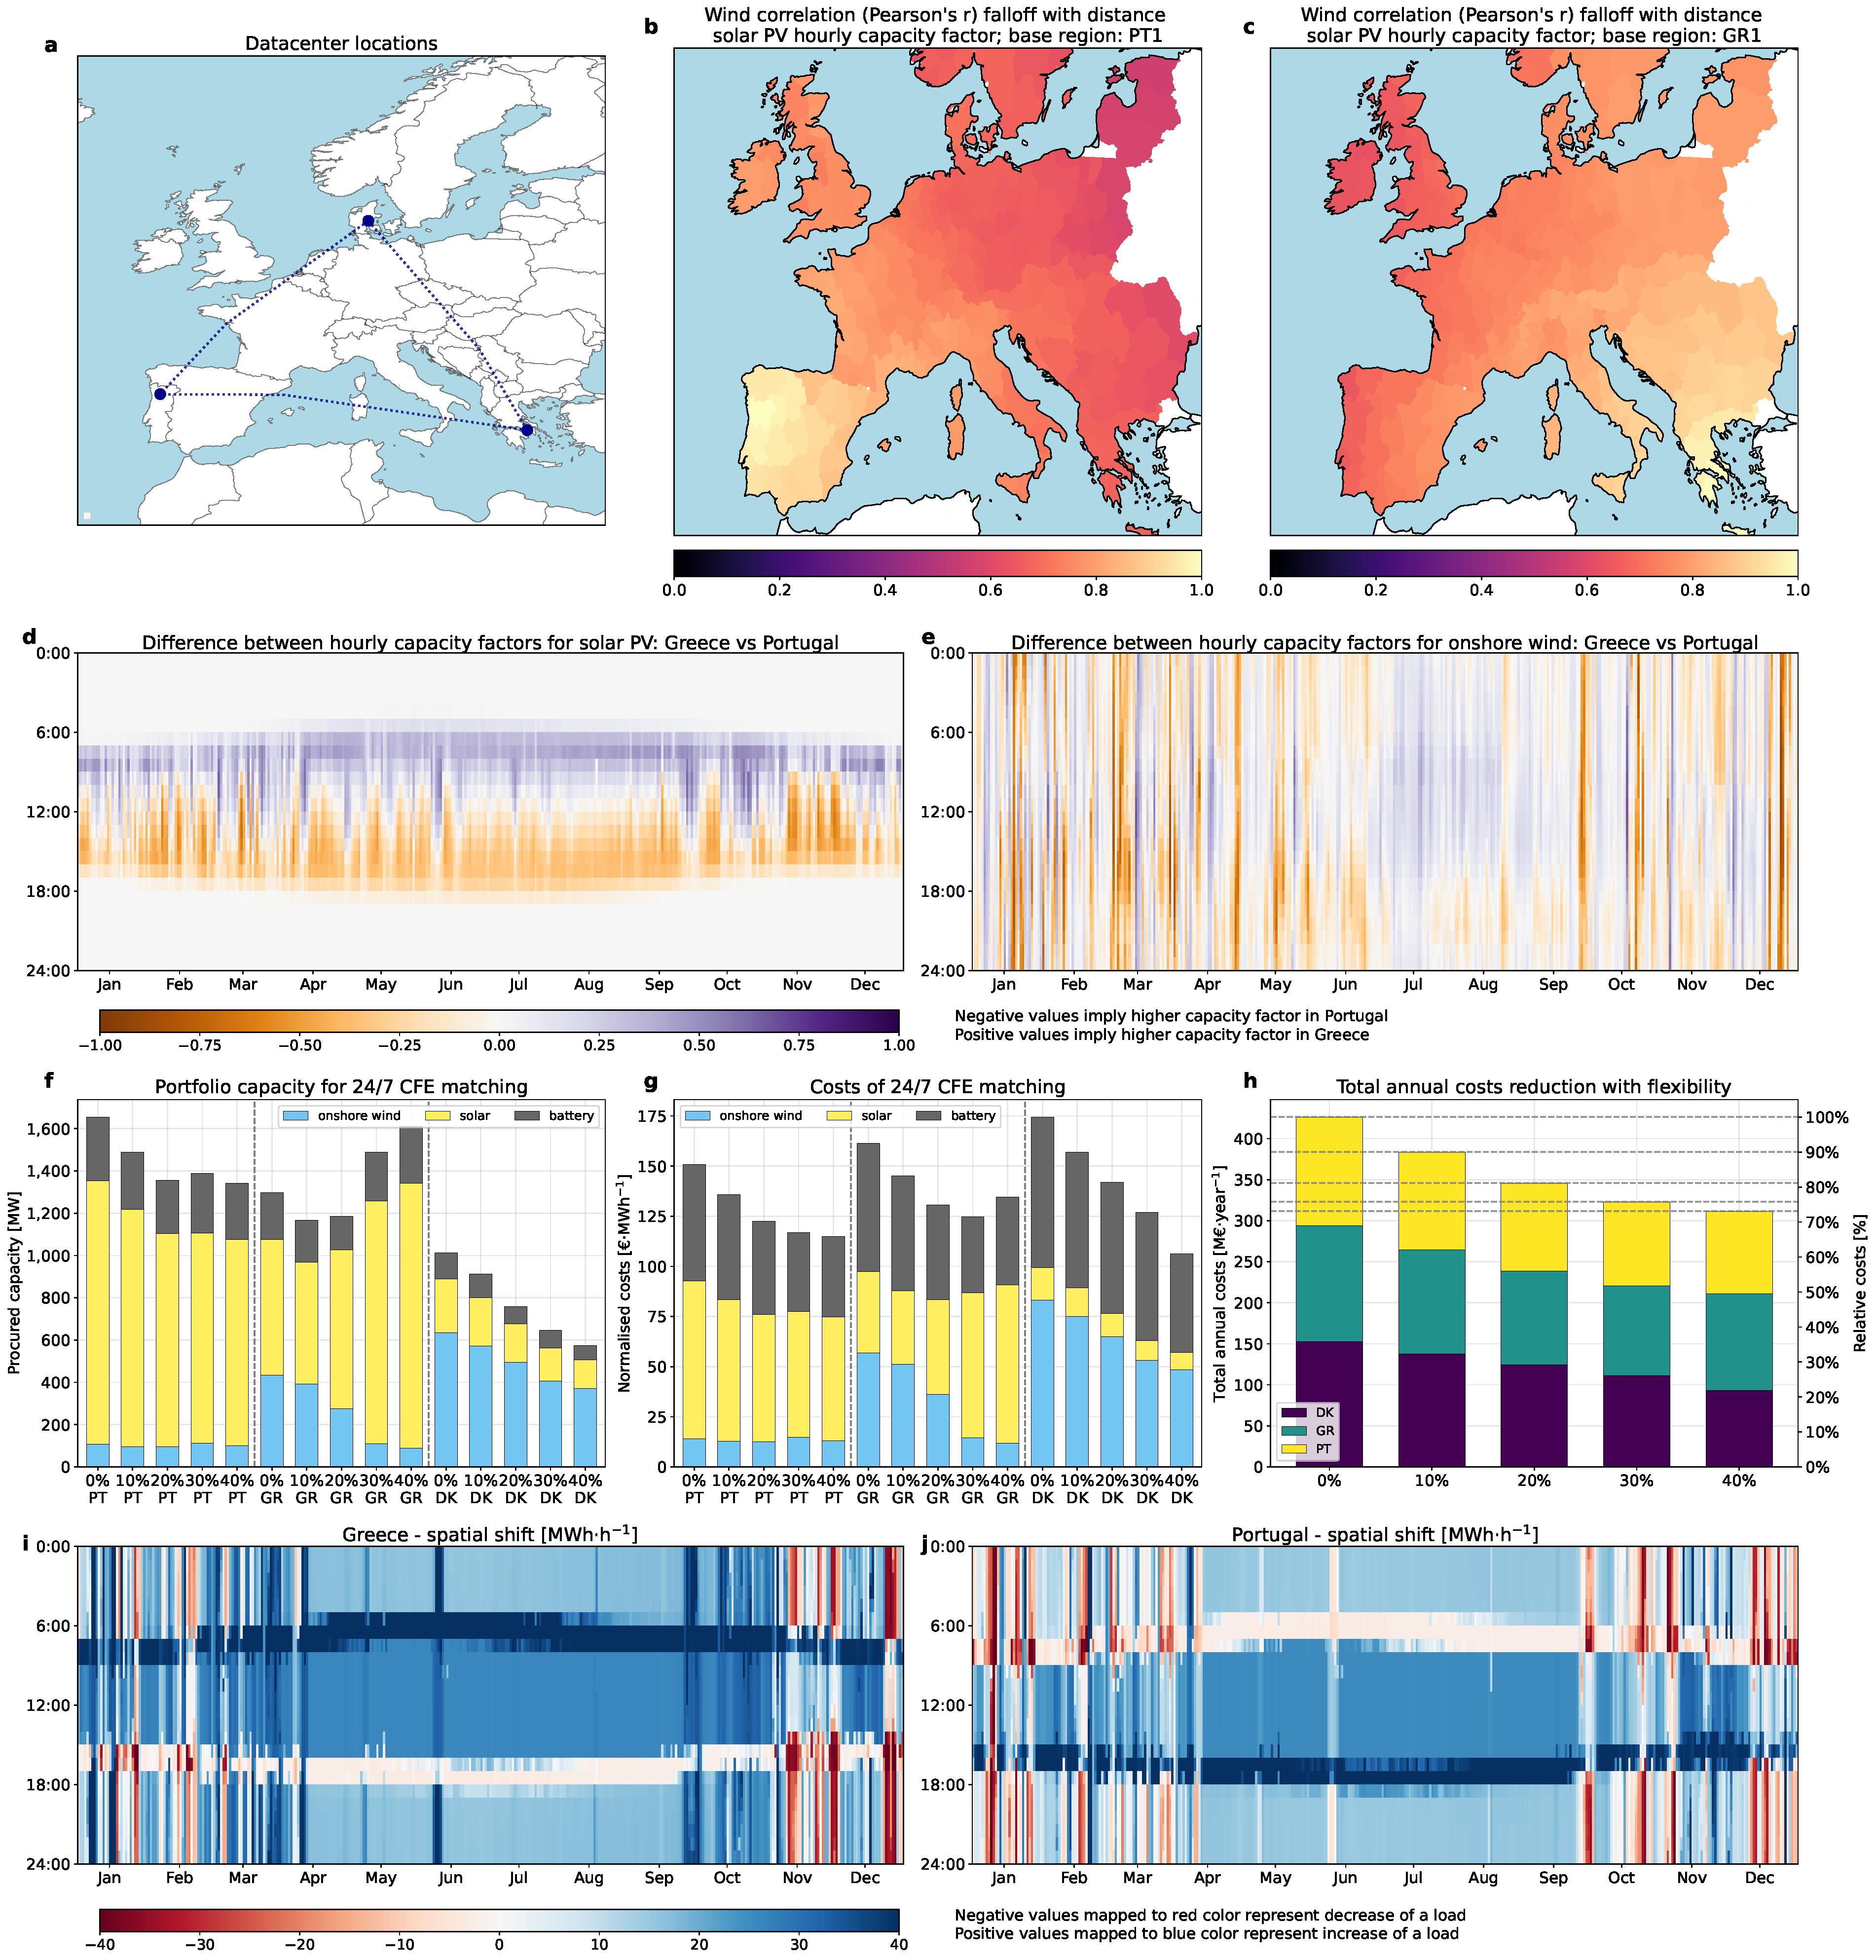
\includegraphics[width=\textwidth]{img/dashboard_3.pdf}
    \caption{Illustration of the signal 3: time lag in solar radiation peaks due to Earth's rotation.
    \textbf{a:} Assumed datacenter locations: Denmark, Portugal, Greece.
    \textbf{b,c:} Peason correlation of hourly capacity factor for solar photovoltaic generation, if selected region of Portugal (panel b) or region of Greece (panel c) is taken as basis. Solar generation remains highly correlated over long distances, in contrast to wind generation.
    \textbf{d:} Difference in solar photovoltaic hourly capacity factors between two selected locations: Greece and Portugal. The two locations are approx. 2700~km apart, which results in a noticeable lag in solar generation peaks due to Earth's rotation.
    \textbf{e:} Difference in wind generation hourly capacity factors between two selected locations: Greece and Portugal. As expected, low correlation of wind feed-in over long distance results in stochastic pattern.
    \textbf{f:} Cost-optimal portfolio of renewable resources and battery storage sufficient for 24/7 matching. Steps on x-axis represent increasing share of flexible load.
    \textbf{g:} Cost breakdown of 24/7 matching strategy.
    \textbf{h:} Total annual costs of 24/7 matching strategy as a function load flexibility. Relative axis is normalized to the costs of inflexible load.
    \textbf{i,j} Hourly spatial load shifts for the selected datacenter locations: Greece (panel i) and Portugal (panel j). Color mapping represents the quantity of load \enquote{received} from other locations or \enquote{sent} away.}
    \label{fig:dashboard3}
\end{figure*}

\subsection{Generalising the results beyond specific load locations}

\begin{figure}
    \centering
    \includegraphics[width=1\columnwidth]{img/flexibility_vs_normalized_costs.pdf}
    \caption{\lipsum[1]}
    \label{fig:flexcost}
\end{figure}
